\chapter{iBEMS Architecture}
\label{ch: Chapter2}


At the center of the iBEMS architecture is the iBEMS core. This core interacts
with multiple peripherals including IoT devices and a weather API over the
internet. Over the course of this project, we managed to develop support for 2
IoT devices displayed in Figure~\ref{fig:highLevelArchitecture}. %
%
\begin{figure}
  \centering
  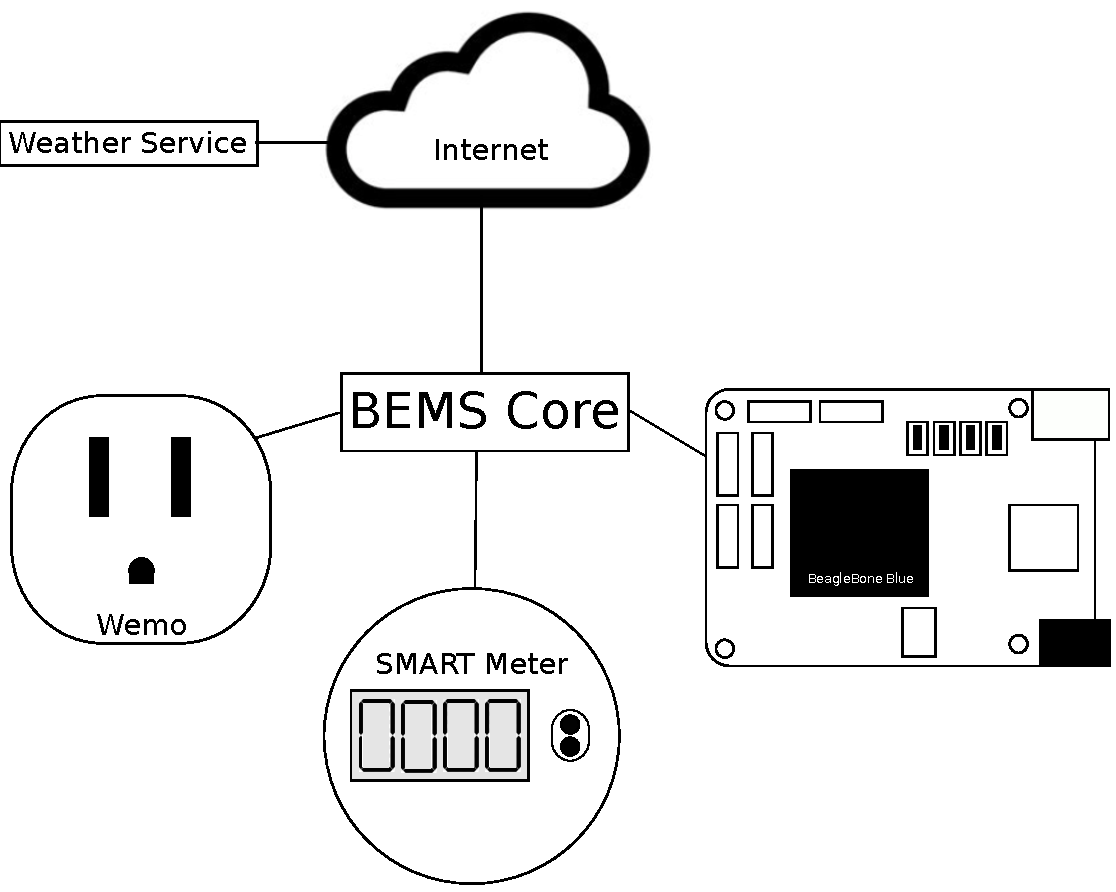
\includegraphics[scale=0.3]{figs/highLevelArchitecture.pdf}
  \caption{High Level Architecture of the Proposed System}
  \label{fig:highLevelArchitecture}
\end{figure}
%
These devices are the WeMo Insight Switch and an embedded computer known as the Beaglebone
Blue. Our initial plan for the smart meter shown in
Figure~\ref{fig:highLevelArchitecture} was to use it in a Simscape model of a
microgrid. However, we did not list this as a requirement for the project, so we
decided not to implement it due to time constraints. The core is also able to
connect the internet to download weather data for Peoria, Illinois through
OpenWeatherMap.

\section{Low Level Architecture}

Figure~\ref{fig:functional_bd} gives lower level detail on the system
architecture. %
%
\begin{figure}
  \centering
  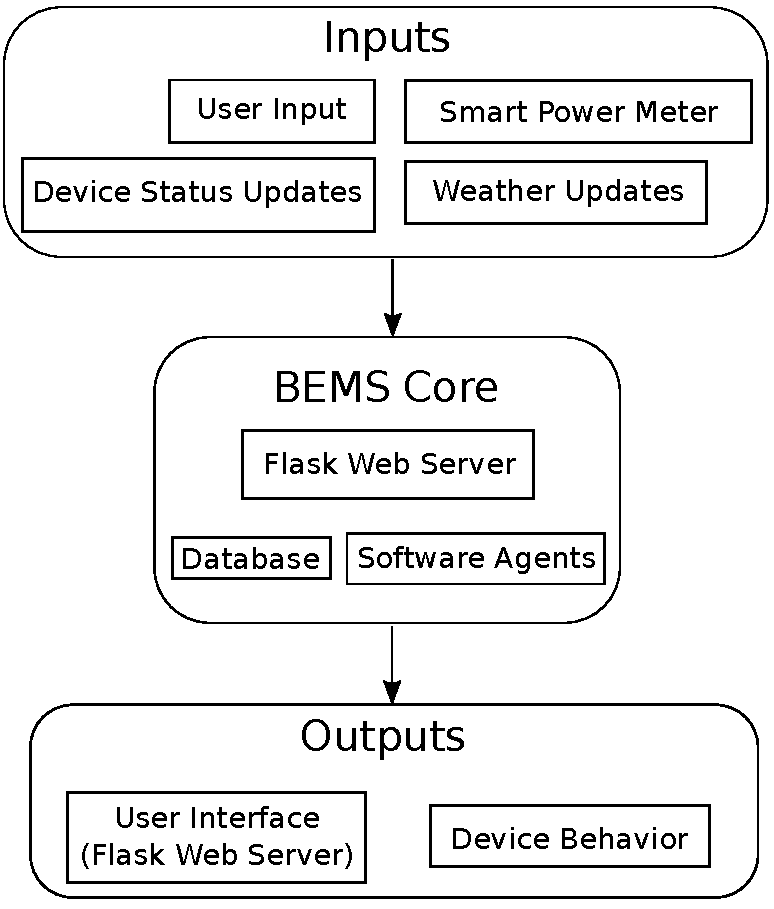
\includegraphics[scale=0.3]{figs/functionalBlockDiagram.pdf}
  \caption{Functional Block Diagram}
  \label{fig:functional_bd}
\end{figure}
%
The inputs include the user input through the web server, the device status
updates (On/Off, power usage, etc...) and the weather data. The iBEMS Core
itself consists of a Flask Web Server, 2 databases (Apache Cassandra and
SQLite), and 3 software agents (Discovery, Control, and Scheduling).


The Flask web server is built using a Python web framework titled Flask which
allows programmers to develop a dynamic web server capable of rendering data to
HTML pages. The benefit of this framework over other Python web frameworks like
Django is the large amount of customization available. For example, the
developers can create a completely custom user login system. For now, the server
is capable of being accessed only on the server computer running Ubuntu Linux.
In the future, support could be added to allow any user on the LAN to access the
web server. Other web frameworks use object relational mapping directly to
access the relevant databases. However, our system uses direct queries with both
SQLite and the Cassandra query language to query the databases. \medbreak We used
2 different databases to store information on. The Apache Cassandra database was
better suited for the time series data such as device status and power usage.
This database was therefore utilized a lot by the Control and Scheduling Agents.
The SQLite database hold parameters that do not change over time like device
ID's, IP addresses, and MAC addresses which made it amendable to the processes
in the Discovery Agent. A possible improvement to this project could be to only
utilize 1 database for development simplicity. \medbreak The first agent that is
used by the iBEMS Core on startup is the discovery agent. It is responsible for
reaching out on the network and finding all devices that the iBEMS Core has
support for. This process involves retrieving the following parameters: IP
address, Port number, MAC address, Manufacturer, Name, and API. Once all
available devices are connected, the Control agent is used to change the status
of each device and collect power usage data in real time. Finally, the
scheduling will take input from the user and place the corresponding scheduling
periods in the Apache Cassandra database. Then, a thread is created to poll the
current device status at regular intervals and update the status if it does not
match the defined status in the Apache Cassandra database.


Figure~\ref{fig:systemComponentInterconnection} provides an explanation of how
the components of the system interact with each other. %
%
\begin{figure}
  \centering
  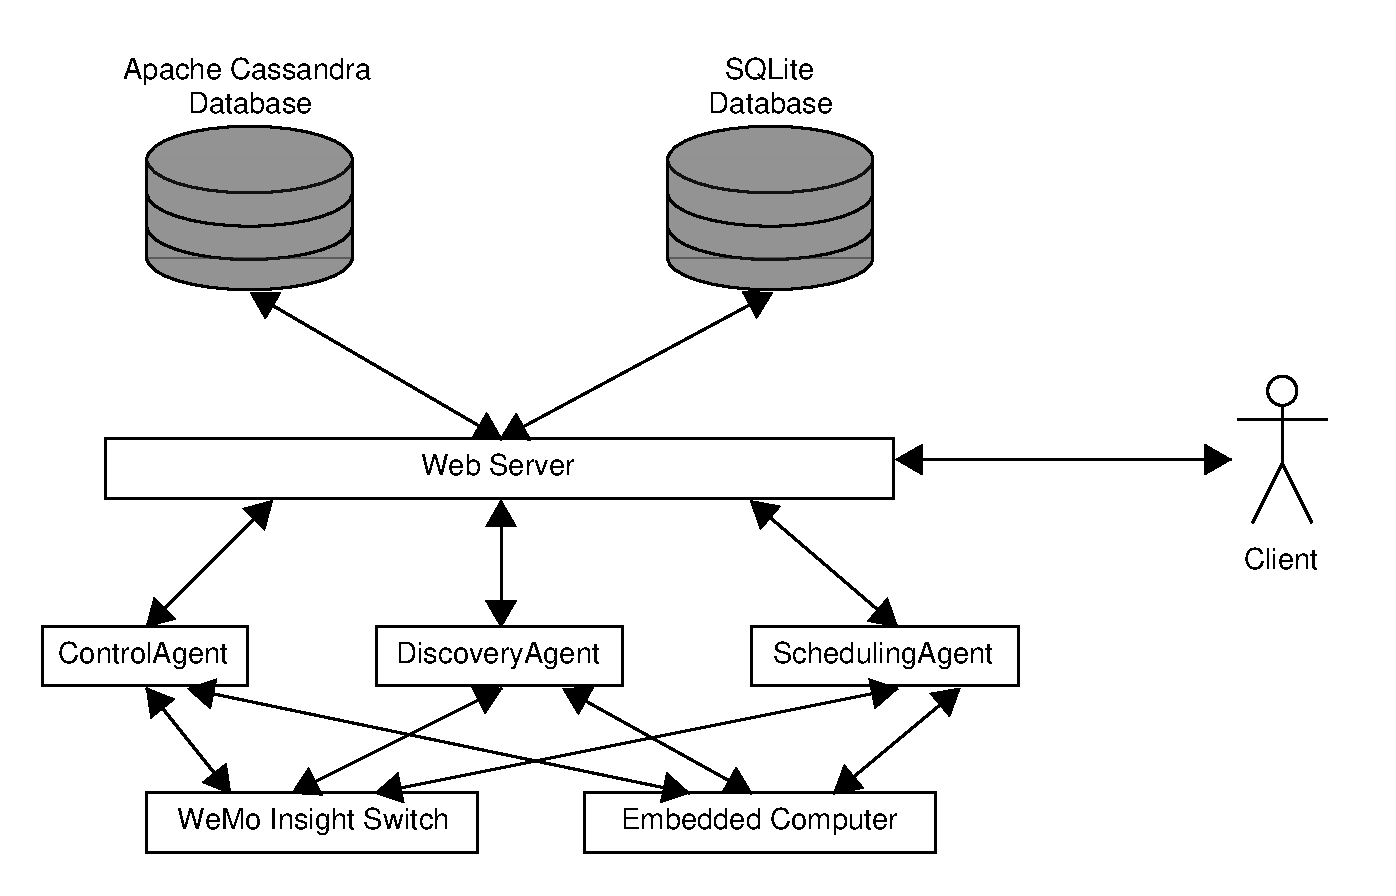
\includegraphics[scale=0.6]{figs/overallDiagram.pdf}
  \caption{Interconnection between system components}
  \label{fig:systemComponentInterconnection}
\end{figure}
%
The Apache Cassandra database and SQLite database are accessible from the web server, control agent, discovery agent, and scheduling agent. The web server queries the time series database and metadata database for vastly different purposes. Power plotting requires querying the Apache Cassandra database. To distinguish between the different devices on the front end, the metadata database is used. The agents utilize the Apache Cassandra database for storing and extracting time-series data. The agents use the metadata database to distinguish between different devices. 

\section{Modes of Operation}


\begin{figure}
  \centering
  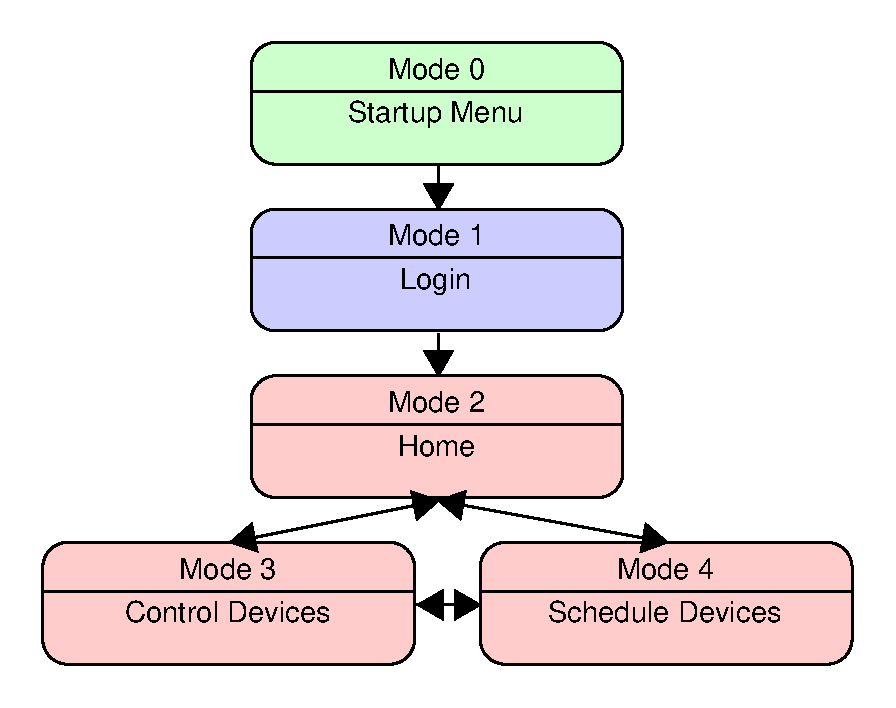
\includegraphics[scale=0.4]{figs/operationalModes.pdf}
  \caption{Operation Modes Interaction}
  \label{fig:operationalModes}
\end{figure}

There are 5 general modes of operation in iBEMS as shown in Figure~\ref{fig:operationalModes}. In Mode 0, before iBEMS is even launched, the user must open the Startup Menu, which is a desktop graphical user interface (GUI). This is a simple GUI with only 2 buttons for starting and stopping iBEMS. Upon clicking \say{Start iBEMS}, the login page will load where the user can enter a valid username and password to use iBEMS. Once a valid username and password is entered, the home screen will be shown which displays the weather data being downloaded from the OpenWeatherMap API. This information includes temperature in Fahrenheit and Celsius, wind speed in MPH, humidity, and cloud coverage. At this point, a navigation bar is available to view the \say{Active Devices} page and the \say{Scheduling} page. \say{Active Devices} corresponds to Mode 3 for controlling devices in real time. The user will also be able to view power plots in this mode as well. Lastly, the \say{Scheduling} page is Mode 4 for creating schedules for all connected devices.

\section{Hardware}

A large feature of this project was being able to record power usage from the
connected IoT devices. The embedded computer does not have a built-in capability
to measure its own power usage, so a circuit was needed to make that
possible. Essentially, this circuit will measure the current being used to drive
one of the motors on the robot chassis. The on-board Analog-to-Digital-Converter
(ADC) can be used to read the voltage across the resistor and since the
resistance is known, the current can be calculated as $I = V/R$. Also, the
voltage from the H-Bridge to drive the motors on the embedded computer is known
so the power consumed by 1 motor is $Motor Drive Voltage * I$. For the specific
robot chassis used in this project, there are 4 motors, so multiplying the power
found from this circuit by 4 will give an approximation of the total power used
by the robot. \add{For other robots with different power sources besides a Lipo
battery.} See Figure~\ref{fig:motorInterfaceCircuit} for details of the interface
circuit for computer power usage by the DC motor. 

\begin{figure}
  \centering
  \begin{circuitikz}[american]
    \tikzstyle{every node} = [font = \tiny]
    % \usetikzlibrary{patterns}
    \draw
    (0,0) to[sqV,invert,l=Motor Drive Voltage from H-Bridge] ++(0,4*\smgrid)
    to[Telmech=M,n=motor,fill=red!20] ++(4*\smgrid,0)
    to[C,l=$1~{[}\mu F{]}$,*-*] ++(0,-4*\smgrid) to[short]++(-4*\smgrid,0); 
    \draw
    (4*\smgrid,4*\smgrid) to[short,-*]++(3*\smgrid,0)
    to[short,-o]++(2*\smgrid,0)node[right]{Embedded Computer ADC (Ch\#0)};
    \draw
    (7*\smgrid,4*\smgrid) to[R,l=$2~{[}\Omega{]}$,-*]++(0,-4*\smgrid)
    to[short]++(-4*\smgrid,0);
    \draw
    (7*\smgrid,0) to[short,-o]++(2*\smgrid,0) node[right]{Embedded
      Computer ADC (Ground)};
  \end{circuitikz}
  \caption{Interface circuit to calculate power consumption of a DC motor
    running from the embedded computer copmuter.}
  \label{fig:motorInterfaceCircuit}
\end{figure}


% \pagebreak
\begin{figure}[H]
    \centering
    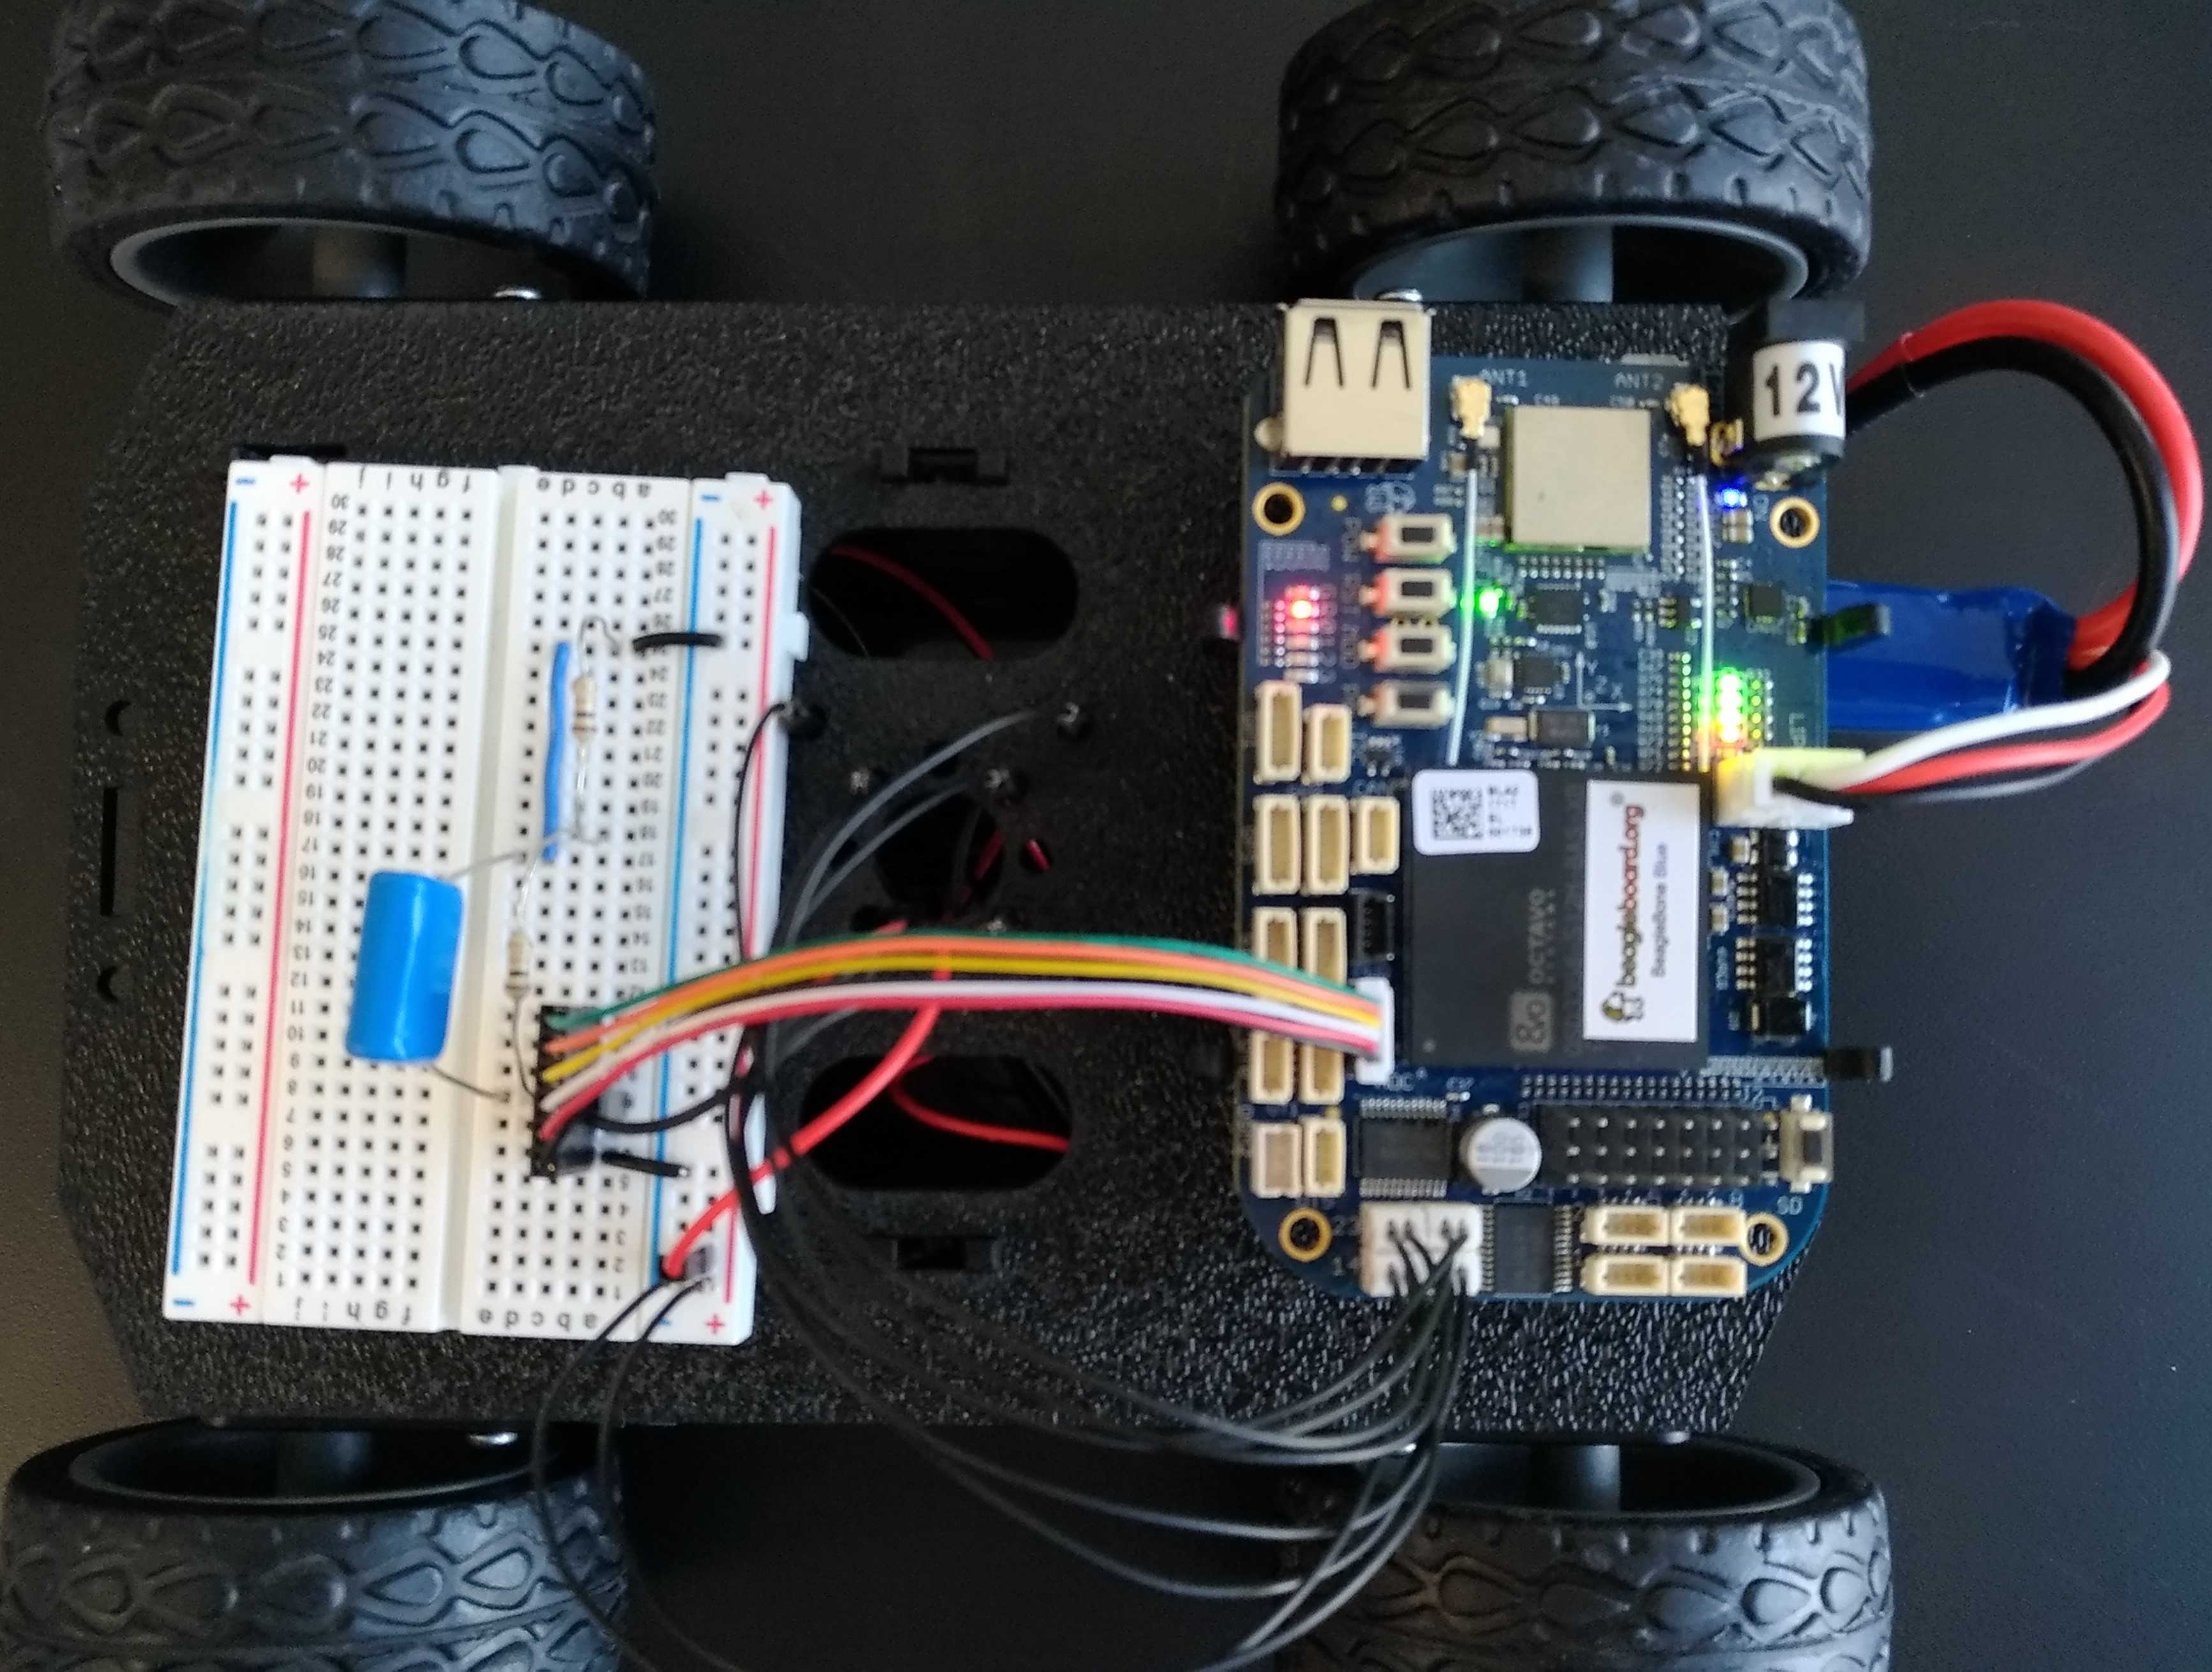
\includegraphics[scale=0.1]{figs/beaglebone/notConnectedSBC.jpg}
    \caption{Embedded Computer Not Connected}
    \label{fig:not_connected_bb}
\end{figure}

Figure~\ref{fig:not_connected_bb} shows the embedded computer mounted on the robot chassis with the circuit shown on page 9. It can also be seen that the embedded computer lights up the on-board red LED when disconnected. Figure~\ref{fig:connected_bb} shows that the embedded computer lights up the green LED when it is connected as an extra indication of its connection status.

\begin{figure}[H]
    \centering
    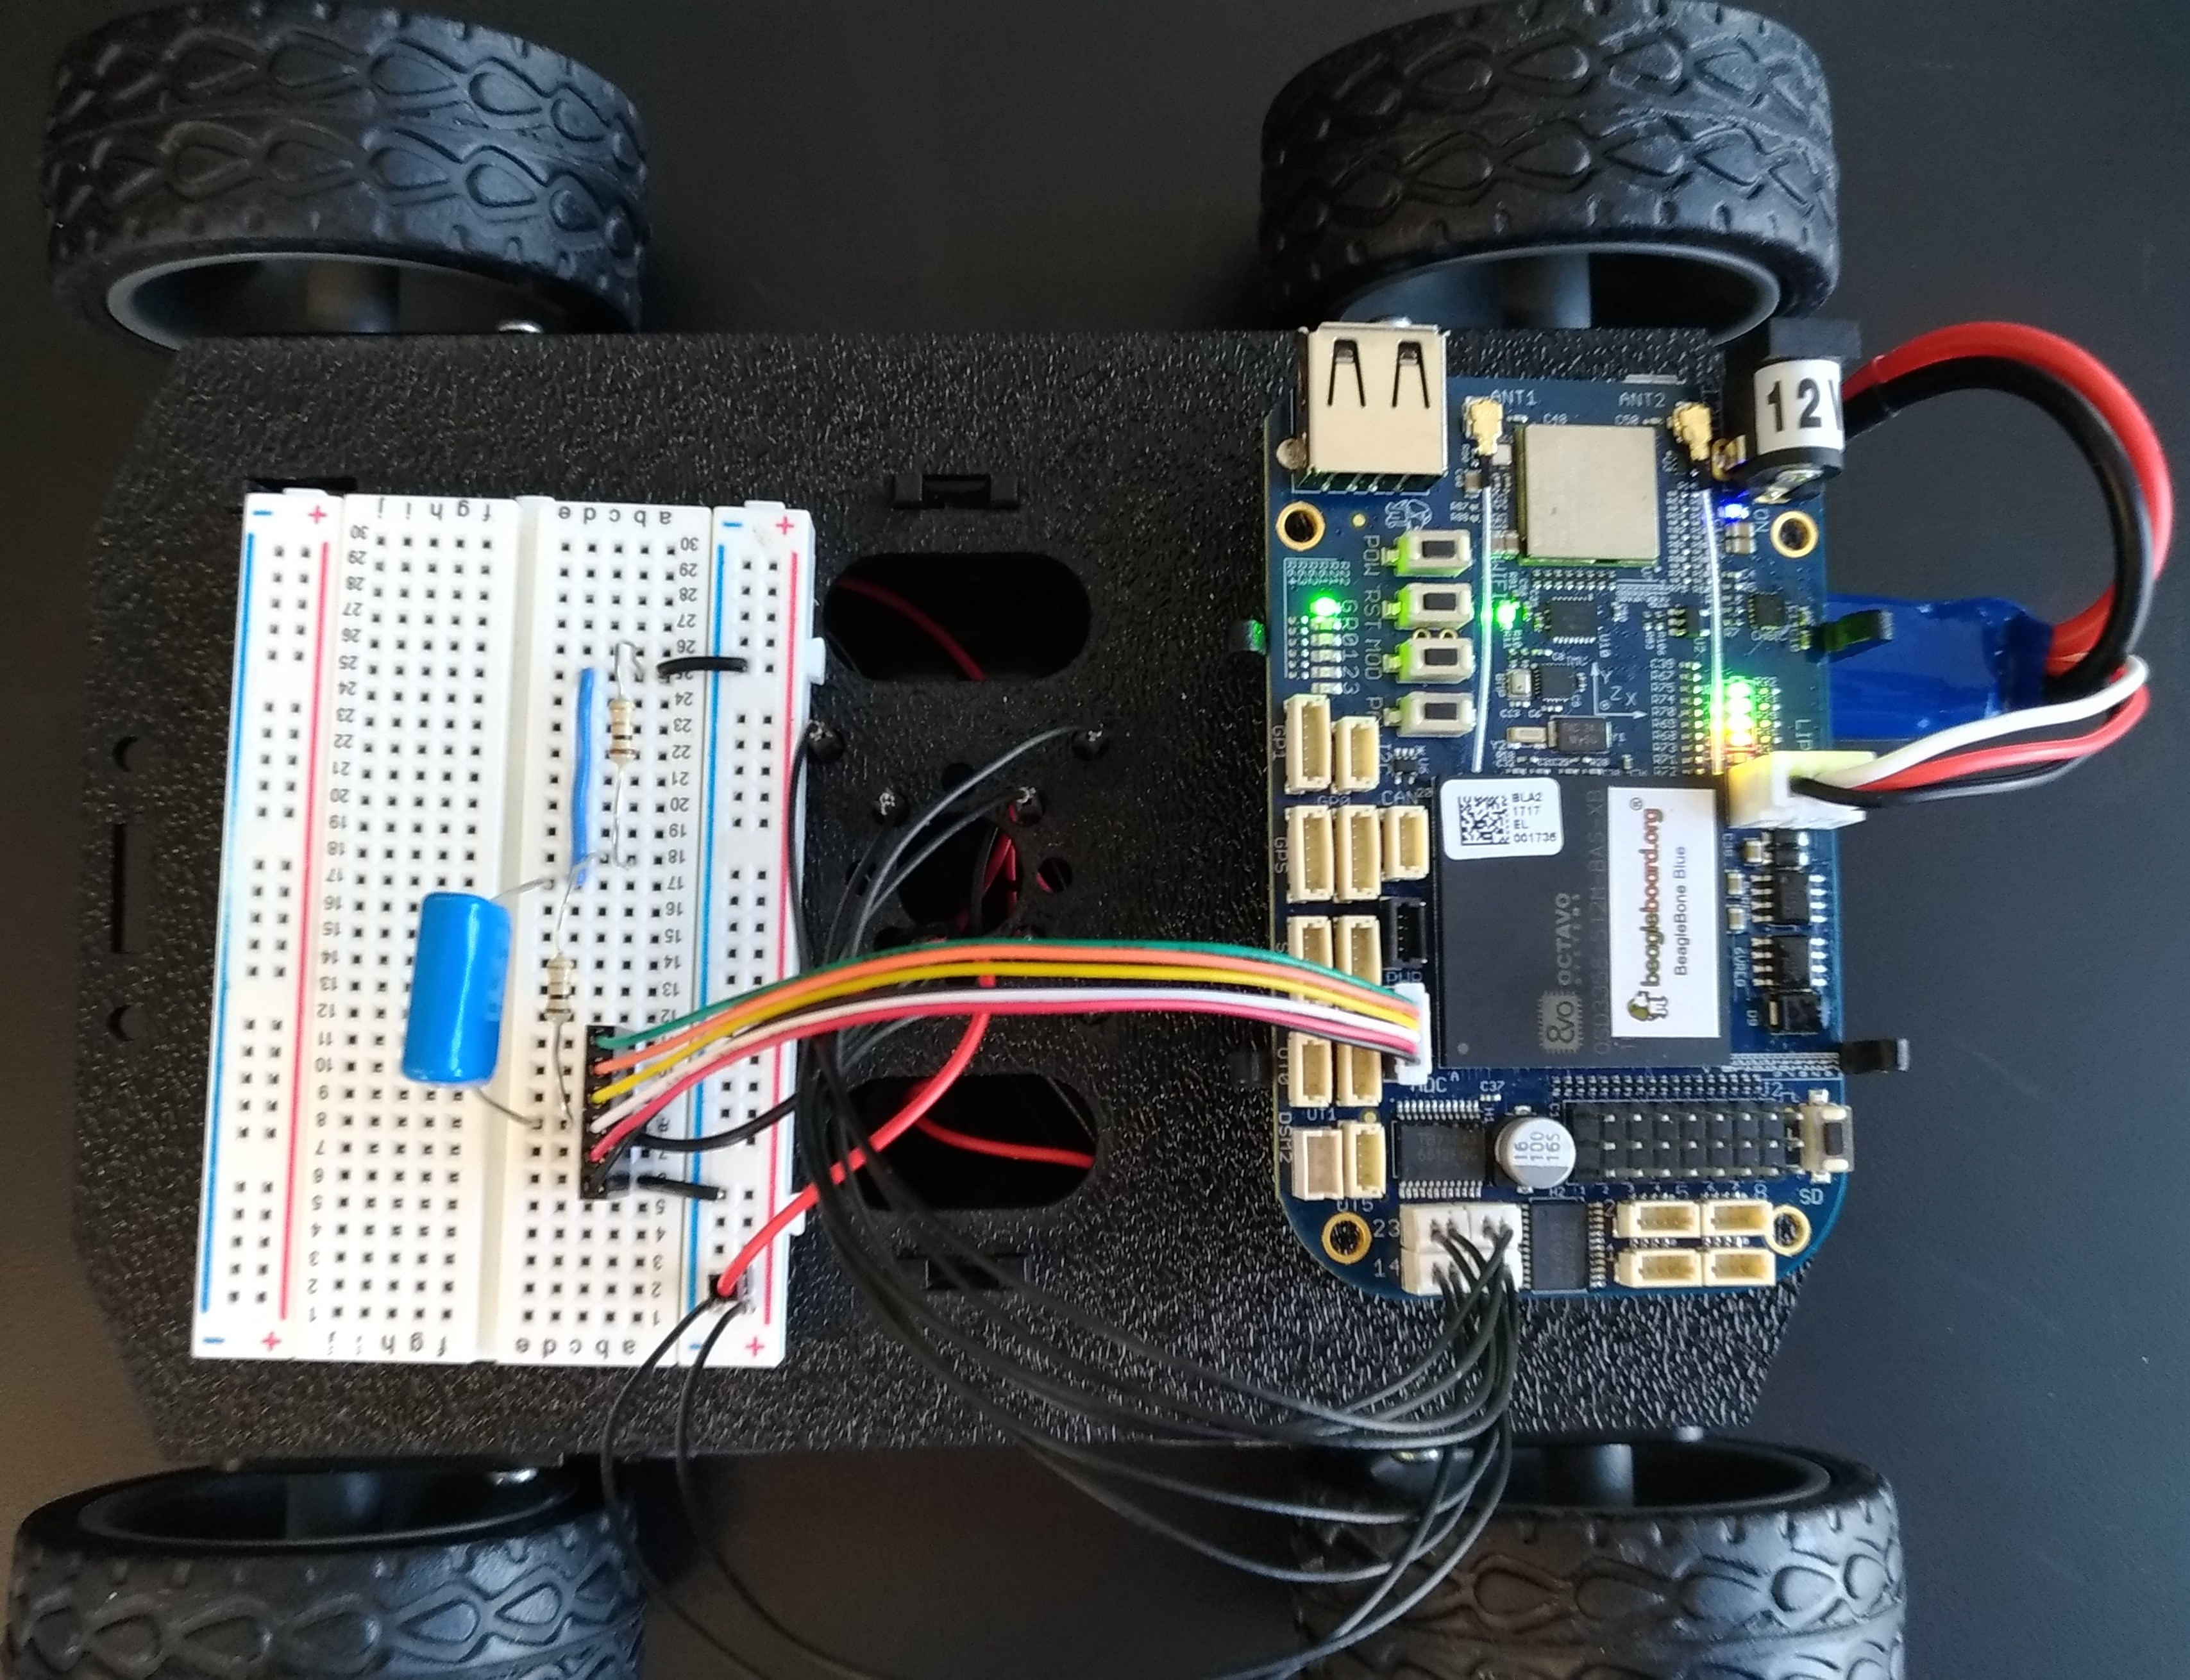
\includegraphics[scale=0.1]{figs/beaglebone/connectedSBC.jpg}
    \caption{Embedded Computer Connected}
    \label{fig:connected_bb}
\end{figure}

\begin{figure}[H]
    \centering
    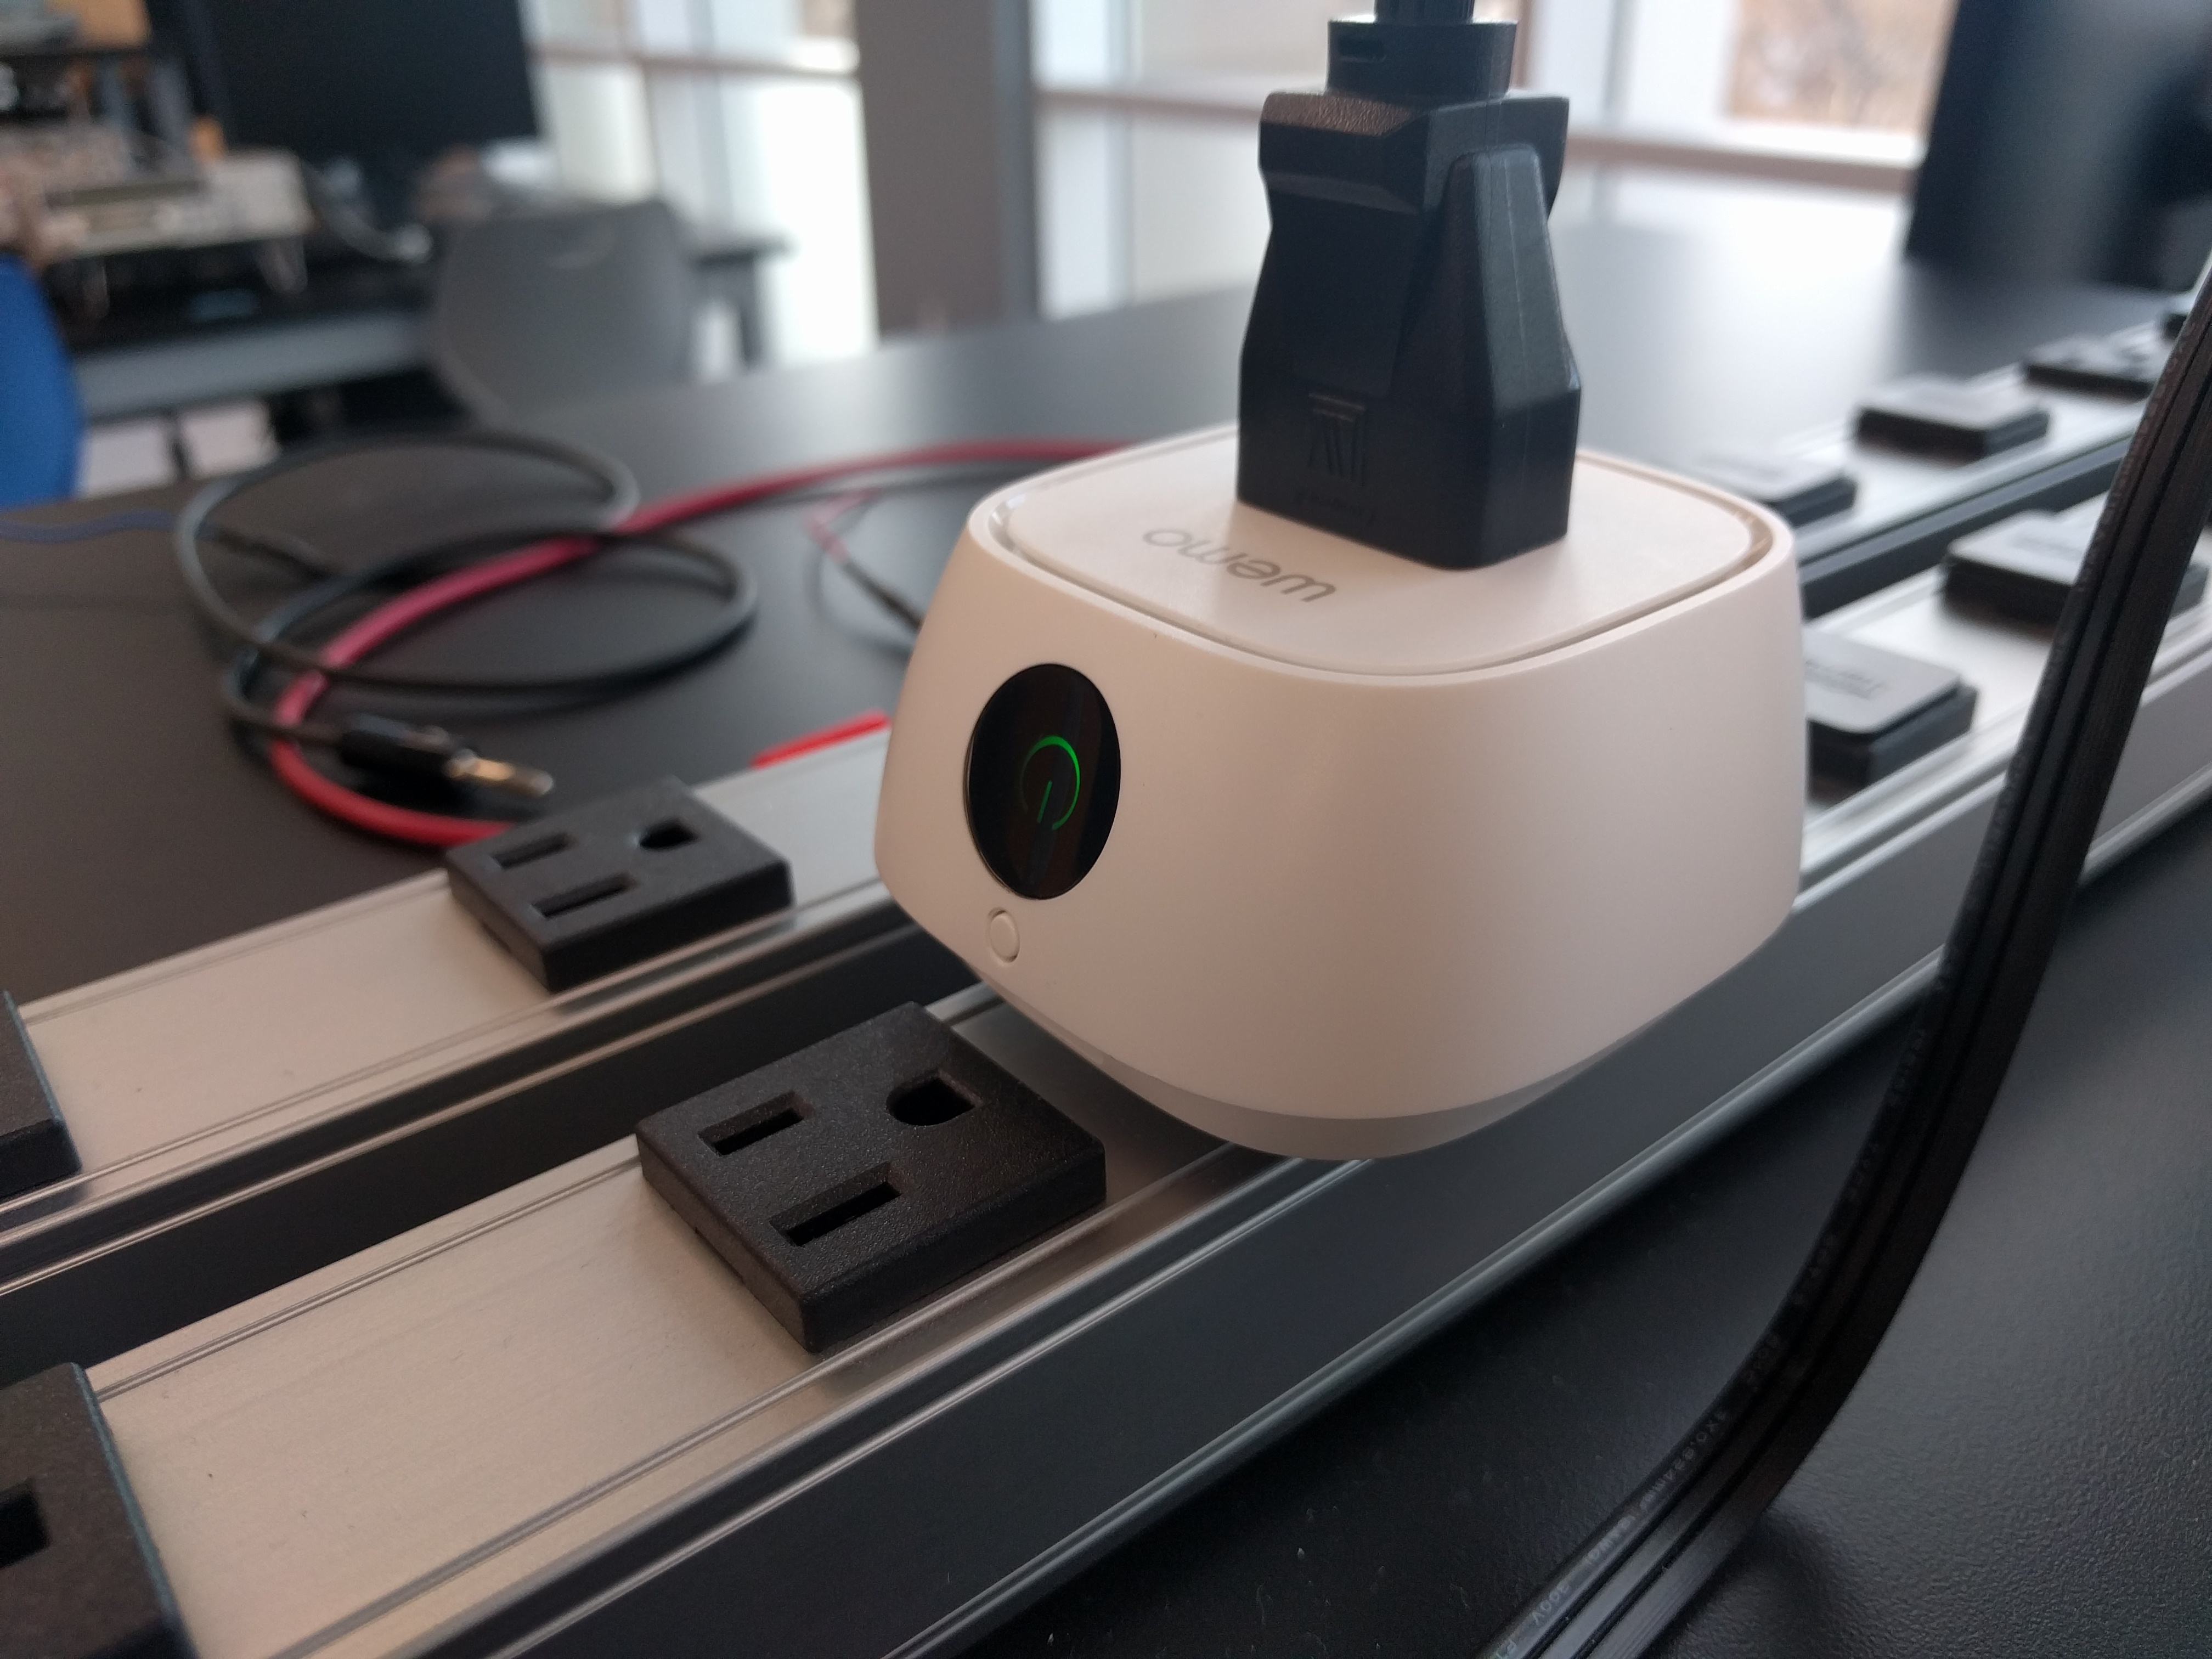
\includegraphics[scale=0.085]{figs/wemo/wemoView.jpg}
    \caption{WeMo Insight Smart Plug}
    \label{fig:wemo}
\end{figure}

The other supported device is the WeMo Insight Switch as seen in Figure~\ref{fig:wemo}. This device was easy to develop support for as it is meant for building energy management. It simply plugs into a 120 volt 3-prong outlet and any typical household appliance running on 120 volts can be plugged into it. Internal circuitry allows the WeMo to be controlled remotely (turn On/Off) and to record power usage of whatever it is plugged into.

\begin{figure}[H]
    \centering
    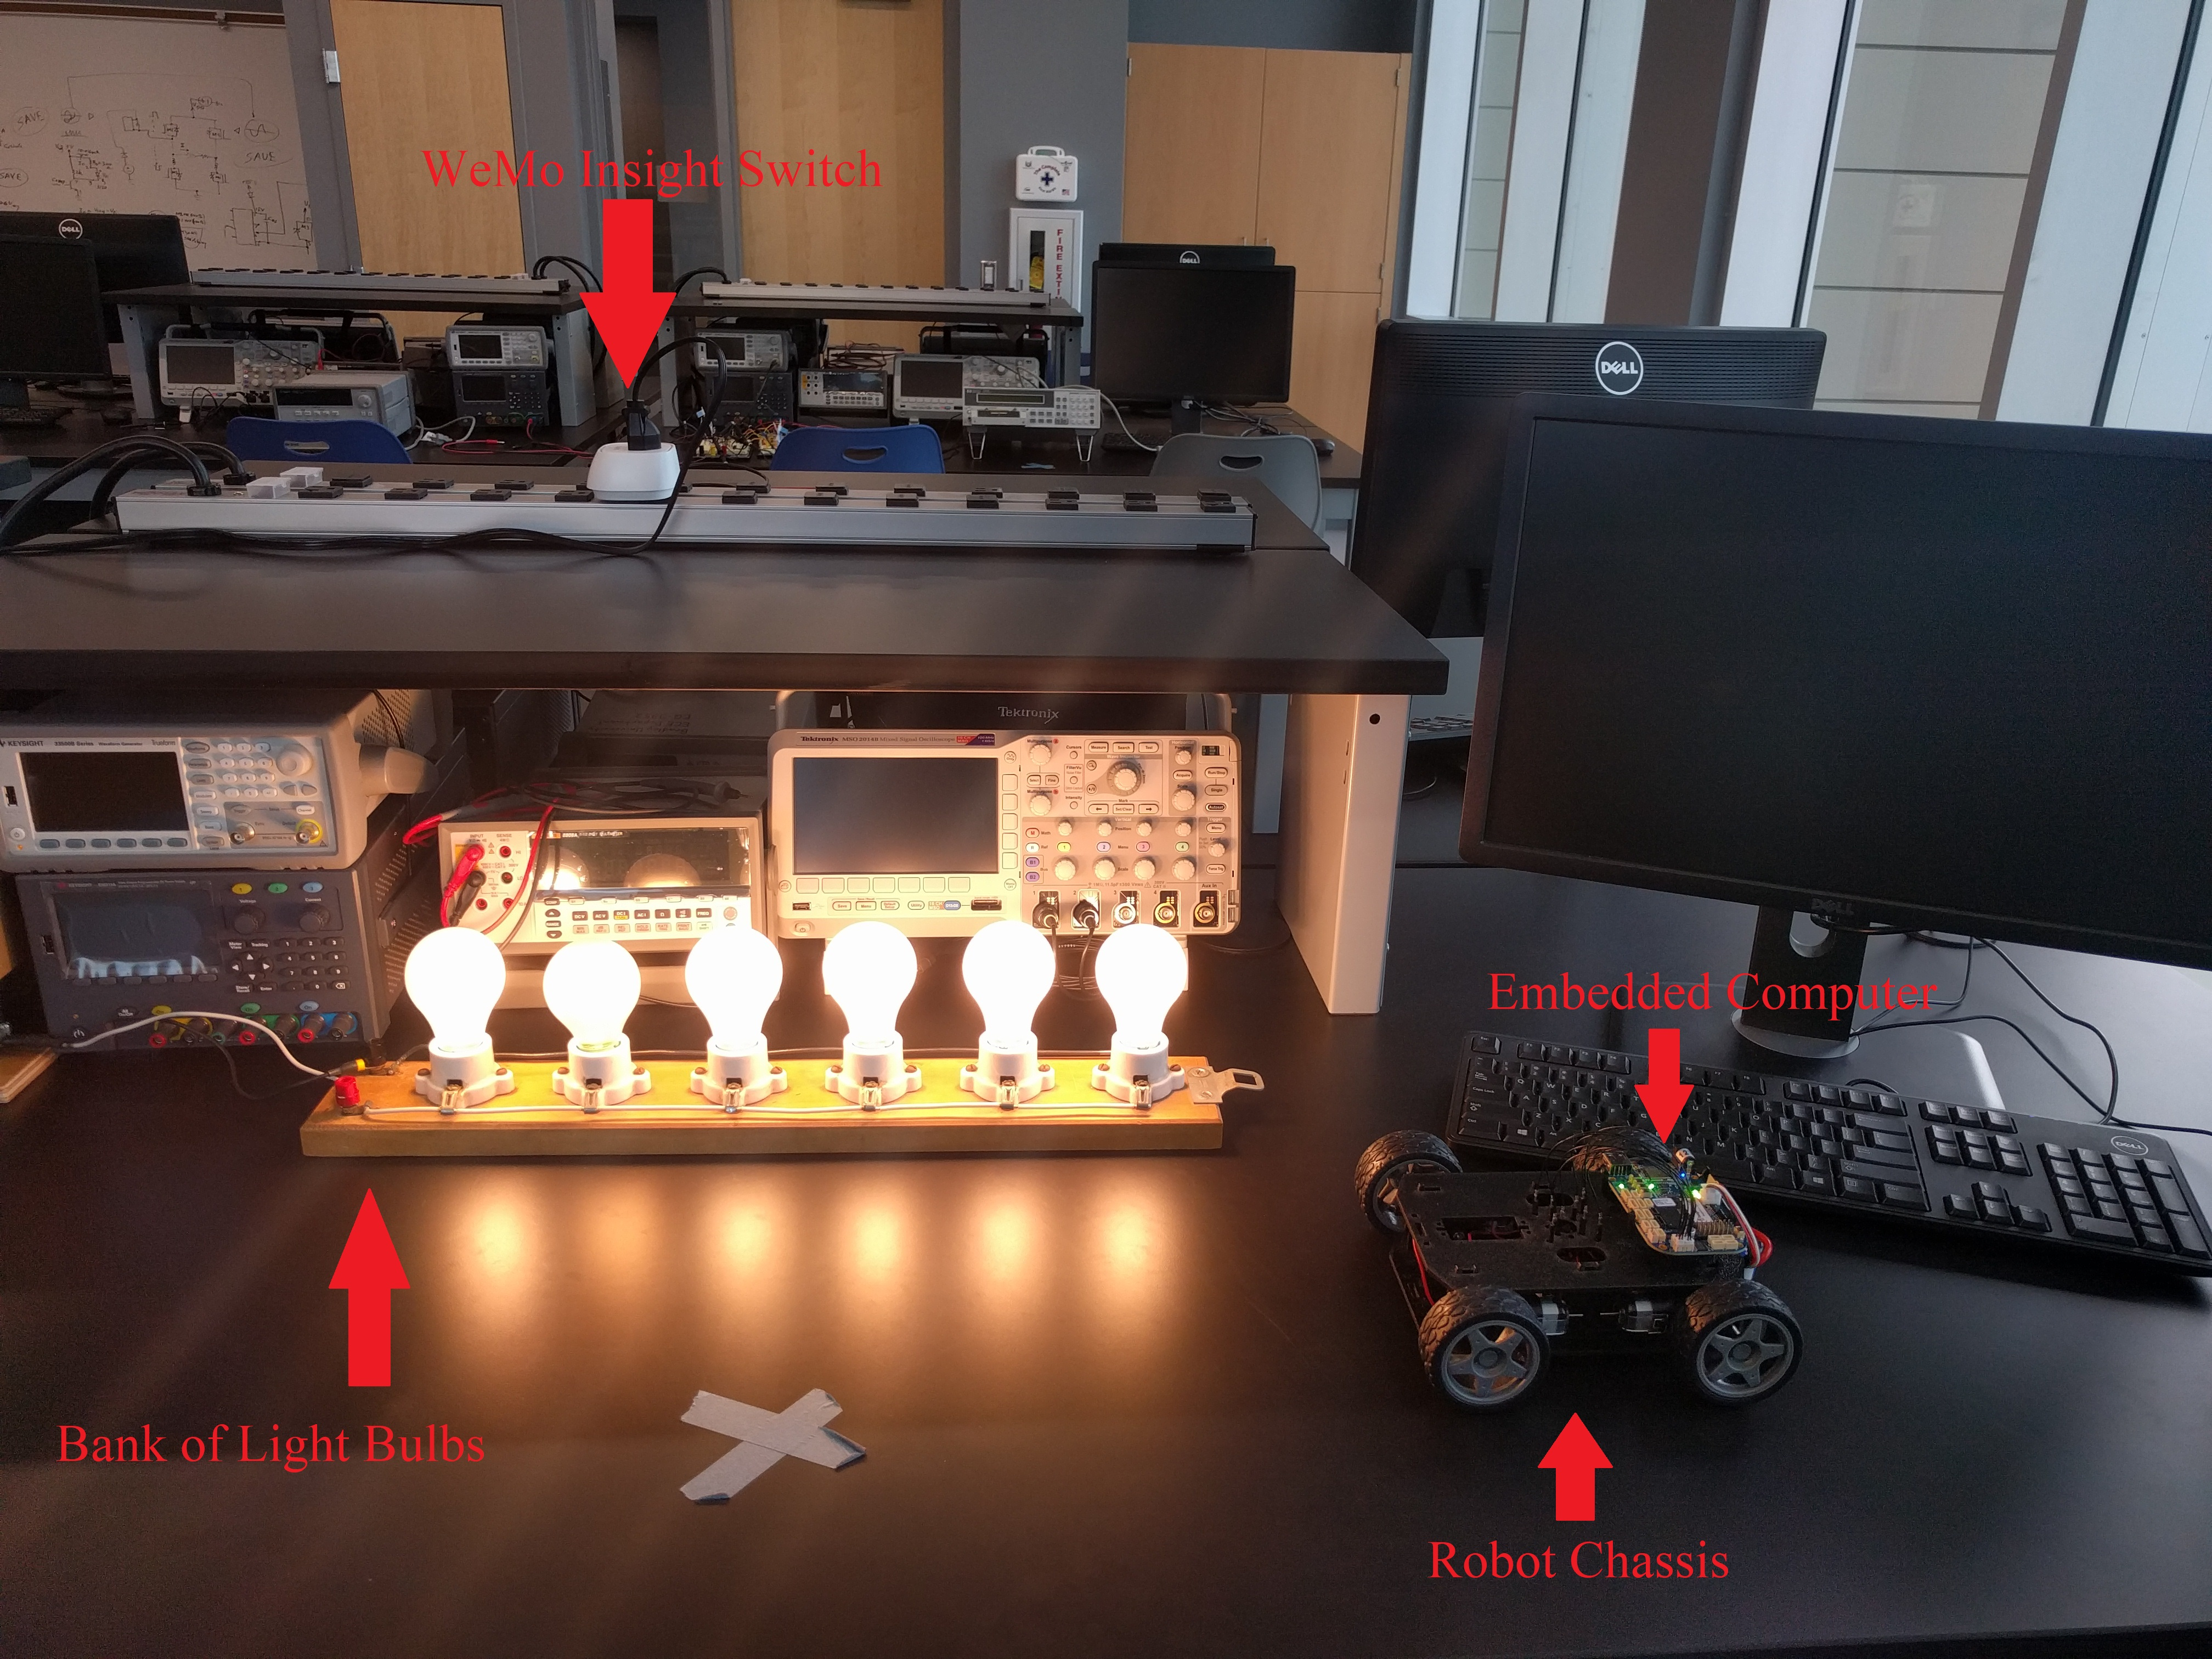
\includegraphics[scale=0.1]{figs/overallView.jpg}
    \caption{Overall View}
    \label{fig:overallView}
\end{figure}

In order to test these devices, we plugged a bank of 6 light bulbs into the WeMo
Insight Switch as seen in Figure~\ref{fig:overallView}. The embedded computer's
functionality was tested with the circuit and robot chassis described earlier.

%%% Local Variables:
%%% mode: latex
%%% TeX-master: "../finalReport"
%%% End:
